\documentclass{protokol}
\leftheader{Studium ohybových jevů v laserovém svazku}
\centerheader{}
\rightheader{Tomáš Derner}

\begin{document}

  \section*{Úkol}

    \begin{enumerate}
      \item Ze změřeného ohybového obrazce zobrazeného na milimetrovém papíru určete mřížkovou konstantu mřížky.
      \item Pomocí aparatury proměřte ohybové obrazce: mřížky, štěrbiny a dvojštěrbiny. Konkrétní difrakční prvky vybere vyučující. Zpracováním měření určete parametry použitých difrakčních prvků.
      \item Okalibrujte mikroskopový okulár s použitím metody lineární regrese, odhadněte relativní chybu kalibrace.
      \item Mikroskopem změřte parametry všech použitých difrakčních prvků.
      \item Výsledky měření v úkolech č.1, č.2 a č.4 srovnejte a diskutujte, v kterém případě jsou spočtené parametry zatíženy nejmenší chybou. 
    \end{enumerate}

  \section*{Teorie}

    V tomto praktiku měříme ohyb laserového svazku způsobený difrakční mřížkou a štěrbinami. Protože použitý laser má poměrně velkou divergenci svazku, použijeme v měření spojnou čočku, viz \cite{mereni}. 

    Pro získání mřížkové konstanty $a_m$ využijeme vztahu pro úhel $\varphi$ mezi dvěma body maximální intenzity difrakčního obrazce
    \begin{equation} \label{eq:mrizkova_konstanta}
      \varphi = \frac{\lambda}{a_m},
    \end{equation} 
    kde $\lambda$ je vlnová délka použitého světla. Úhel $\varphi$ získáme z rovnice
    \begin{equation} \label{eq:phi}
      \varphi = \frac{x}{l},
    \end{equation}
    kde $x$ je vzdálenost dvou maxim a $l$ vzdálenost difrakčního obrazce od spojné čočky. 

    Pro úhel mezi sousedními dvěma body minimální intenzity světla difrakčního obrazce štěrbiny a obálky obrazce dvojštěrbiny platí vztah
    \begin{equation} \label{eq:sterbina}
      \varphi = \frac{\lambda}{b},
    \end{equation}
    kde $b$ je šířka štěrbiny,
    pro úhel mezi dvěma minimy obrazce dvojštěrbiny pak platí obdobný vztah
    \begin{equation} \label{eq:dvojsterbina}
      \varphi = \frac{\lambda}{a},
    \end{equation}
    kde $a$ je vzdálenost středů štěrbin. Pro úhel $\varphi$ platí také vztah \eqref{eq:phi}, kde $x$ je nyní vzdálenost sousedních minim.

  \section*{Výsledky}

    Vzdálenost difrakčních obrazců od čočky byla 
    $$ l = \SI{1.000 \pm 0.005}{m}, $$
    vlnová délka použitého světla byla 
    $$ \lambda = \SI{632.8}{nm}. $$

    \subsection*{Úkol 1}

      V tabulce \ref{tab:u1} jsou zaneseny vzdálenosti sousedních maxim difrakčního obrazce difrakční mřížky odečtené z milimetrového papíru.

      \begin{table}[H]
        \centering
        \setlength{\tabcolsep}{2.6pt}
        \begin{tabular}[t]{
  lSSSSSSSSSSSSSSSSSSSSS
}\toprule
x [mm] & 1.3 & 1.2 & 1.2 & 1.3 & 1.2 & 1.2 & 1.2 & 1.3 & 1.2 & 1.2 & 1.3 & 1.2 & 1.2 & 1.3 & 1.2 & 1.2 & 1.2 & 1.3 & 1.2 & 1.2 & 1.3 \\\bottomrule
\end{tabular}
        \caption{Vzdálenosti mezi maximy difrakčního obrazce mřížky}
        \label{tab:u1}
      \end{table}

      Průměrná vzdálenost dvou sousedních maxim byla 
      $$ x = \SI{1.23 \pm 0.05 e-2}{m}. $$

      Pomocí vztahů \eqref{eq:mrizkova_konstanta} a \eqref{eq:phi} jsme získali mřížkou konstantu
      $$ a_m = \SI{5.13 \pm 0.10 e-5}{m}. $$

    \subsection*{Úkol 2}

      Intenzita světla vynesená v grafech níže nabývá hodnot 0 - 255 a popisuje odezvu snímače na dopadající světlo.

      V grafu \ref{fig:mrizka} je zobrazen difrakční obrazec difrakční mřížky. Odečtením poloh peaků a použitím vzorce \eqref{eq:mrizkova_konstanta} a \eqref{eq:phi} jsme dostali mřížkovou konstantu 
      $$ a_m = \SI{5.20 \pm 0.05 e-5}{m}. $$

      \begin{figure}[H]
        \centering
        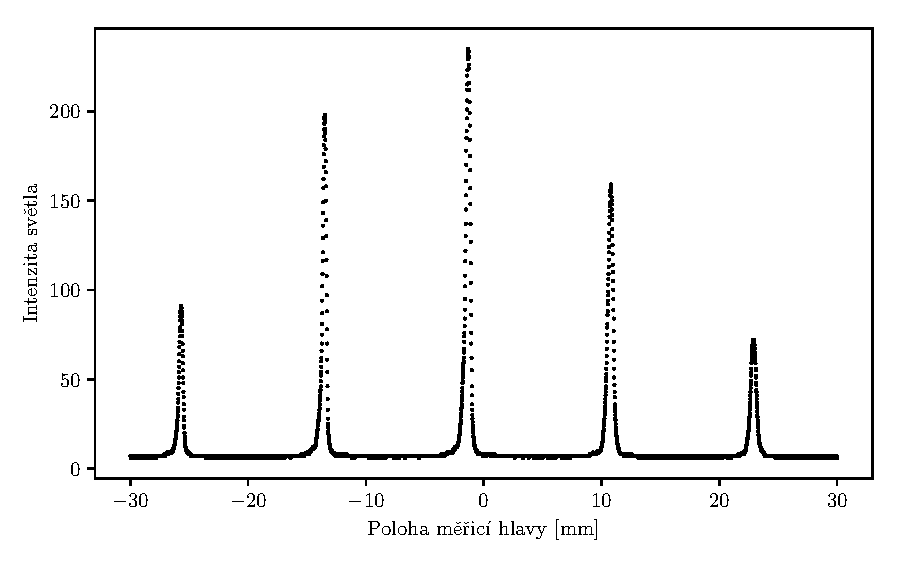
\includegraphics[]{mrizka} 
        \caption{Difrakční obrazec mřížky}
        \label{fig:mrizka}
      \end{figure}

      \begin{figure}[H]
        \centering
        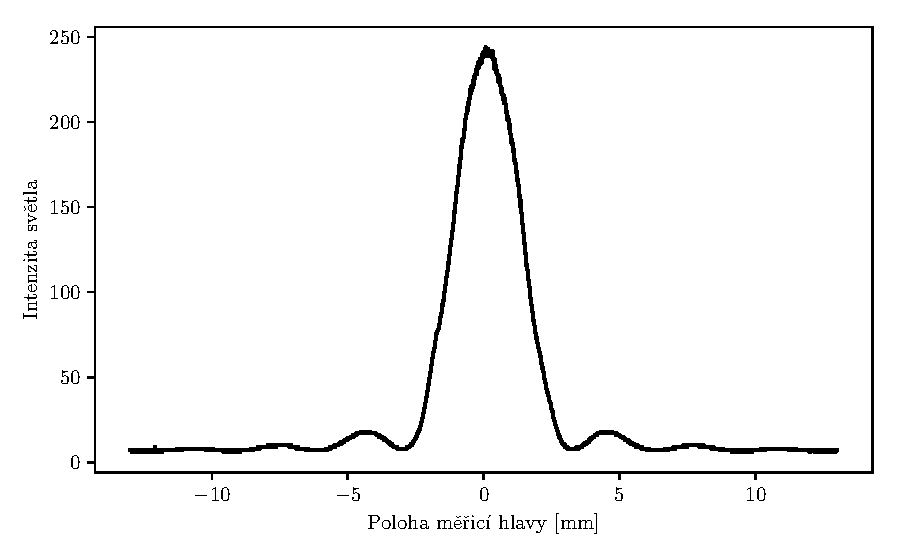
\includegraphics[]{sterbina_stredni}
        \caption{Difrakční obrazec štěrbiny}
        \label{fig:sterbina_stredni}
      \end{figure}

      \begin{figure}[H]
        \centering
        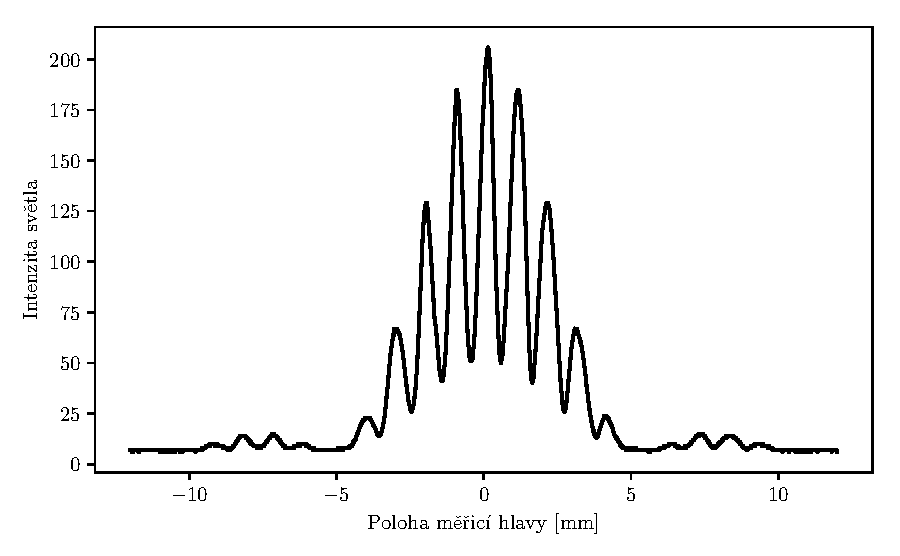
\includegraphics[]{dvojs_blizke}
        \caption{Difrakční obrazec dvojštěrbiny}
        \label{fig:dvojs_blizke}
      \end{figure}

      Použitím průměrné hodnoty poloh minim z grafu \ref{fig:sterbina_stredni} ve vztahu \eqref{eq:phi} a \eqref{eq:sterbina} dostaneme šířku štěrbiny 
      $$ b = \SI{2.05 \pm 0.02 e-4}{m}. $$
      
      Obdobným použitím vztahu \eqref{eq:dvojsterbina} pro minima grafu \ref{fig:dvojs_blizke} dostaneme vzdálenost štěrbin
      $$ a = \SI{6.00 \pm 0.09 e-4}{m}. $$

      Obálka tohoto grafu nemá dostatečný počet zřetelných minim pro použití předešlé metody, vzdálenostem susedních minim jsou však ekvivalentní vzdálenosti minim prvního řádu od maxima řádu nultého. Použitím těchto hodnot ve vztahu \eqref{eq:phi} a \eqref{eq:sterbina} dostaneme šířky štěrbin 
      $$ b_d = \SI{1.18 \pm 0.02 e-4}{m}. $$

    \subsection*{Úkol 3}

      Byla provedena kalibrace měřítka mikroskopu metodou postupných měření. Data byla zpracována lineární regresí, směrnice regrese je $\num{6.10 \pm 0.01}$. Jeden dílek na stupnici mikroskopu tedy odpovídá $\frac{1}{\num{6.10}}$ milimetrům, relativní chyba kalibrace činí $\pm \SI{0.2}{\percent}$.

      \begin{figure}[H]
        \centering
        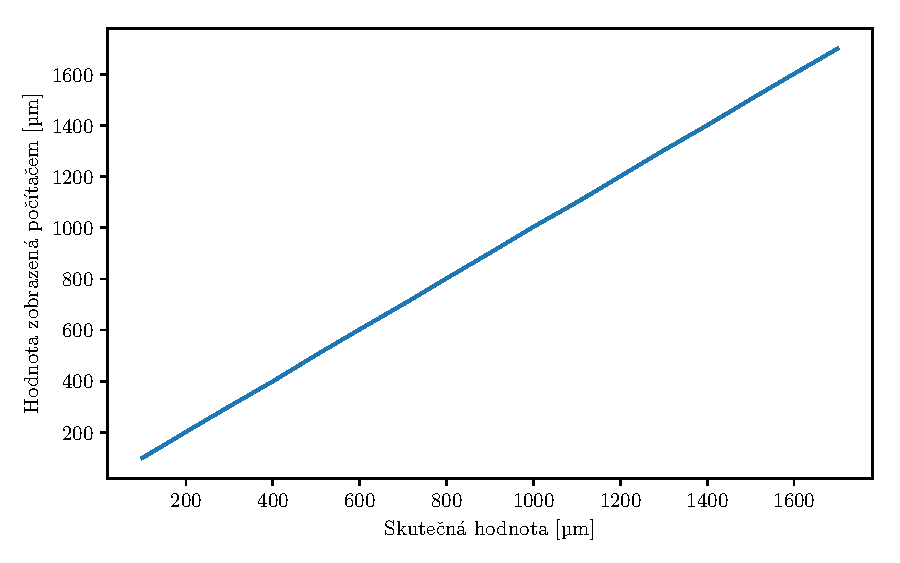
\includegraphics[]{kalibrace}
        \caption{Kalibrace stupnice mikroskopu}
        \label{fig:kalibrace}
      \end{figure}

    \subsection*{Úkol 4}

      Pomocí mikroskopu jsme získali rozměry použitých optických prvků, tabulka \ref{tab:mrizka} obsahuje vzdálenosti deseti vrypů mřížky, tabulka \ref{tab:sterbina_stredni} šířku štěrbiny na třech místech a tabulka \ref{tab:dvojs_blizke} šířku a vzdálenost štěrbin na třech místech.

      \begin{table}[H]
        \centering
        \setlength{\tabcolsep}{10pt}
        \begin{tabular}[t]{
  S[table-format=1.2]
  S[table-format=1.2]
  S[table-format=1.2e1]
} \toprule
{poloha vrypu}       & {vzdálenost od dalšího vrypu} & {vzdálenost od dalšího vrypu} \\
{[dílek mikroskopu]} & {[dílek mikroskopu]}          & {[m]}                         \\\midrule
3.54                 & 0.32                          & 5.24e-5                       \\
3.83                 & 0.29                          & 4.75e-5                       \\
4.16                 & 0.31                          & 5.08e-5                       \\
4.47                 & 0.32                          & 5.24e-5                       \\
4.79                 & 0.31                          & 5.08e-5                       \\
5.10                 & 0.32                          & 5.24e-5                       \\
5.42                 & 0.31                          & 5.08e-5                       \\
5.73                 & 0.33                          & 5.40e-5                       \\
6.02                 & 0.29                          & 4.75e-5                       \\
6.34                 &                               &                               \\\bottomrule
\end{tabular}

        \caption{Hodnoty vzdáleností vrypů mřížky}
        \label{tab:mrizka}
      \end{table}

      Průměrná hodnota vzdálenosti dvou vrypů a tedy i mřížkové konstanty je $$ a_m = \SI{5.09 \pm 0.07 e-5}{m}.$$
      
      \begin{table}[H]
        \centering
        \setlength{\tabcolsep}{5pt}
        \begin{tabular}[t]{
  S[table-format = 1.0]
  S[table-format = 1.2]
  S[table-format = 1.2]
  S[table-format = 1.2]
  S[table-format = 1.2e1]
} \toprule
{měření} & {poloha začátku št.} & {poloha konce št.} & {šířka štěrbiny}     & {šířka štěrbiny} \\
         & {[dílek mikroskopu]}      & {[dílek mikroskopu]}    & {[dílek mikroskopu]} & {[m]}            \\\midrule
1        & 2.50                      & 3.80                    & 1.30                 & 2.13e-4          \\
2        & 2.52                      & 3.81                    & 1.29                 & 2.11e-4          \\
3        & 2.74                      & 2.74                    & 1.24                 & 2.03e-4          \\\bottomrule
\end{tabular}

        \caption{Hodnoty šířky štěrbiny na třech místech}
        \label{tab:sterbina_stredni}
      \end{table}

      Průměrná hodnota šířky štěrbiny je $$ b = \SI{2.09 \pm 0.03 e-4}{m}.$$
      
      \begin{table}[H]
        \centering
        \setlength{\tabcolsep}{10pt}
        \begin{tabular}[t]{
  l
  S[table-format=1.3]
  S[table-format=1.3]
  S[table-format=1.3]
} \toprule
měření                         & {1}   & {2}   & {3}   \\\midrule
začátek první štěrbiny [dílek] & 2.08  & 2.20  & 2.06  \\
konec první štěrbiny [dílek]   & 2.75  & 2.94  & 2.80  \\\midrule
začátek druhé štěrbiny [dílek] & 5.72  & 5.90  & 5.76  \\
konec druhé štěrbiny [dílek]   & 6.46  & 6.75  & 6.51  \\\midrule
šířka první štěrbiny [dílek]   & 0.67  & 0.74  & 0.74  \\
šířka první štěrbiny [mm]      & 0.109 & 0.121 & 0.121 \\\midrule
šířka druhé štěrbiny [dílek]   & 0.74  & 0.85  & 0.75  \\
šířka druhé štěrbiny [mm]      & 0.121 & 0.140 & 0.123 \\\midrule
vzdálenost štěrbin [dílek]     & 3.64  & 3.70  & 3.70  \\
vzdálenost štěrbin [mm]        & 0.596 & 0.606 & 0.606 \\\bottomrule
\end{tabular}

        \caption{Hodnoty šířky a vzdálenosti štěrbin na třech místech}
        \label{tab:dvojs_blizke}
      \end{table}

      Aritmetický průměr vzdálenosti štěrbin je 
      $$ a = \SI{6.02 \pm 0.03 e-4}{m}. $$
      Protože hodnoty šířek štěrbin jsou pro obě štěrbiny téměř shodné, považujeme obě štěrbiny za stejně široké a aritmetický průměr této veličiny počítáme že všech naměřených hodnot. Tento průměr činí 
      $$ b_d = \SI{1.23 \pm 0.04 e-4}{m}. $$


  \section*{Diskuse}

    Všechny hodnoty parametrů difrakčních prvků použitých v tomto měření měřené nepřímou metodou pomocí difrakčních obrazců se v rámci chyby shodují s hodnotami měřenými přímo zkalibrovaným mikroskopem. 
    
    Chybové údaje u hodnot měřených nepřímou metodou jsou o něco menší než u odpovídajících hodnot metody přímé především proto, že při měření difrakcí není snadné odhadnout skutečnou míru nejistoty měření. K tomu dále přistupuje skutečnost, že díky relativně úzkému laserovému svazku se v difrakčním obrazci projevila velmi lokalizovaná hodnota šířky štěrbiny resp. dvojštěrbiny, zatímco mikroskopem byla měřena jejich šířka po celé délce štěrbin.

  \section*{Závěr}

    Z milimetrového papíru byly odečteny polohy maxim difrakčního obrazce difrakční mřížky a pomocí nich spočtena mřížková konstanta 
    $$ a_m = \SI{5.13 \pm 0.10 e-5}{m}. $$
    
    Pomocí aparatury byly změřeny difrakční obrazce mřížky, štěrbiny a dvojštěrbiny.

    Z těchto obrazců byla určena hodnota mřížkové konstanty
    $$ a_m = \SI{5.20 \pm 0.05 e-5}{m}, $$
    šířka štěrbiny 
    $$ b = \SI{2.05 \pm 0.02 e-4}{m}, $$
    šířka obou štěrbin dvojštěrbiny
    $$ b_d = \SI{1.18 \pm 0.02 e-4}{m} $$
    a vzdálenost jejich středů
    $$ a = \SI{6.00 \pm 0.09 e-4}{m}. $$

    Byla provedena kalibrace mikroskopu.

    Zkalibrovaným mikroskopem byly naměřeny parametry použitých prvků:\\
    mřížková konstanta
    $$ a_m = \SI{5.09 \pm 0.07 e-5}{m},$$
    šířka štěrbiny
    $$ b = \SI{2.09 \pm 0.03 e-4}{m},$$
    šířka obou štěrbin dvojštěrbiny
    $$ b_d = \SI{1.23 \pm 0.04 e-4}{m} $$
    a vzdálenost jejich středů
    $$ a = \SI{6.02 \pm 0.03 e-4}{m}. $$

  \begin{thebibliography}{}

    \bibitem{mereni}
    Pokyny k měření "Studium ohybových jevů v laserovém svazku", dostupné z\\ \url{http://physics.mff.cuni.cz/vyuka/zfp/_media/zadani/pokyny/mereni_306.pdf}, 18.\,3.\,2018
  
  \end{thebibliography}

\end{document}